\chapter{System evaluation}
\label{chapter:results}

In an effort to demonstrate the effectiveness of the designed control scheme, an evaluation procedure was developed. This procedure and its results will be explored in this section.


\section{Overview of Experiments}
\label{section:experiment_overview}

The evaluation of the control system was carried out through several experiments designed to assess performance under various trajectory following conditions commonly found in clinical procedures. The experiments were structured to test the system's response within different trajectories. Two primary experiments were developed to evaluate this:

\begin{itemize}
    \item \textbf{Sinusoidal Path Following}: This experiment consisted of a pre-generated sinusoidal path which the robot was required to follow. The path was designed to test the system's ability to track a smooth, continuous trajectory while maintaining stability and accuracy. The period of the sin wave was chosen to rapid changes in desired trajectory velocities that the system might experience. Its amplitude was selected to push the system towards its positional limits in each axis. For the pitch axis a period of 3 seconds with an amplitude of $\pm 15$ degrees was chosen whereas for the roll axis a period of 3 seconds and an amplitude of $\pm 20$ degrees was chosen.
    
    \item \textbf{Target Following}: This experiment was designed to reflect real-world conditions that the subsystems would encounter. In this experiment, first, The MTM was used to generate a target trajectory path that was representative of typical movements during a surgical procedure. Then both axes then attempted to follow this path as closely as possible. The exact 3D trajectory followed during this experiement can be seen in Figure \ref{fig:desired_trajectory}.
\end{itemize}

\begin{figure}[H]
    \centering
    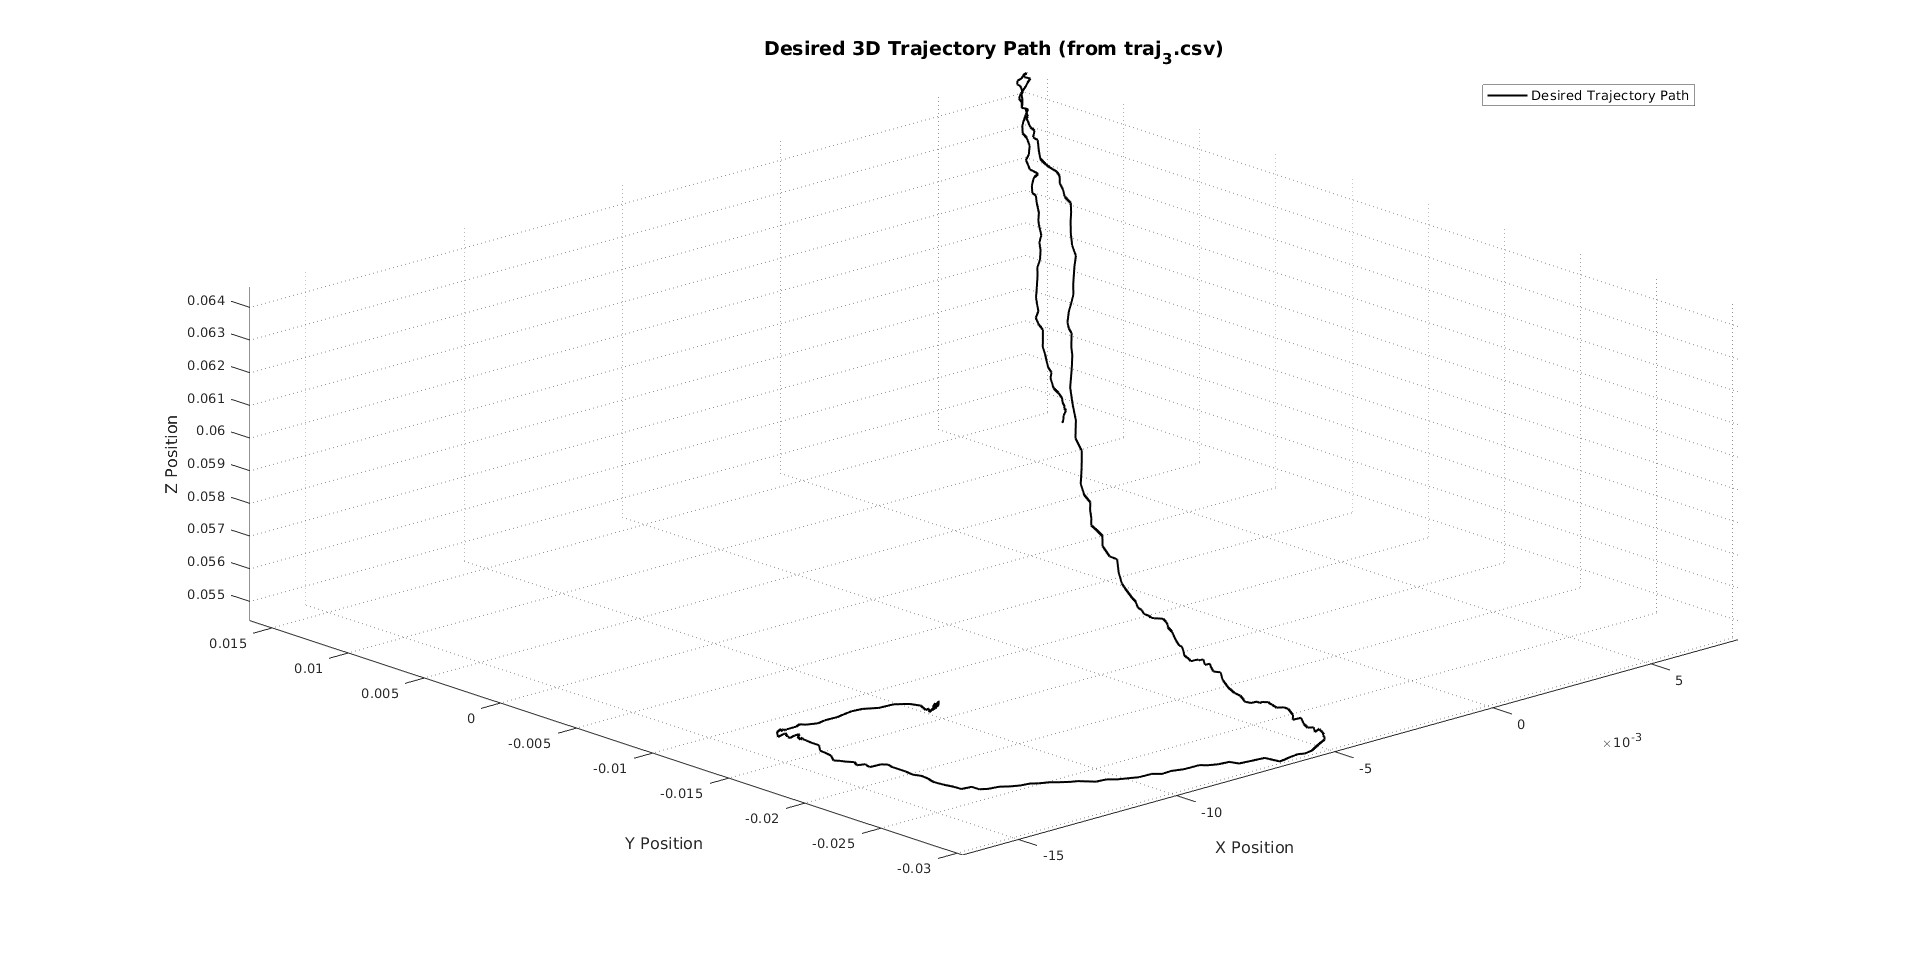
\includegraphics[width=1.0\linewidth]{figures/desired_trajectory.jpg}
    \caption{The 3D trajectory generated by the MTM, representing a typical surgical movement for target following experiments.}
    \label{fig:desired_trajectory}
\end{figure}

During these experiments, the control scheme during this research was tested alongside the previously developed control scheme. During each trial, the target position, actual positions, commanded motor speed, and positional error were carefully tracked and logged. This data was then parsed using a custom MATLAB script and plotted to compare the performance of the two control algorithms. The following sections detail the results of these experiments, focusing on trajectory tracking performance and the effect of the control algorithm on the system's overall performance.

\section{Control Algorithm Performance}
\label{section:trajectory_performance}

These experiments revealed a significant increase in performance for the new control algorithm. It was observed during both the sinusoidal path-following and trajectory-following experiments that the positional error was greatly reduced in both the roll and pitch axes. 

\subsection{Sinusoidal Path Following Experiment Results}

With the previous proportional control algorithm, the system consistently undershot or overshot the target position and lagged behind the intended trajectory, particularly at the extrema of the joint angles. This is highlighted in Figure \ref{fig:roll_p_sin} and Figure \ref{fig:pitch_p_sin}, which show the system's performance during sinusoidal path following with proportional control.

\begin{figure}[H]
    \centering
    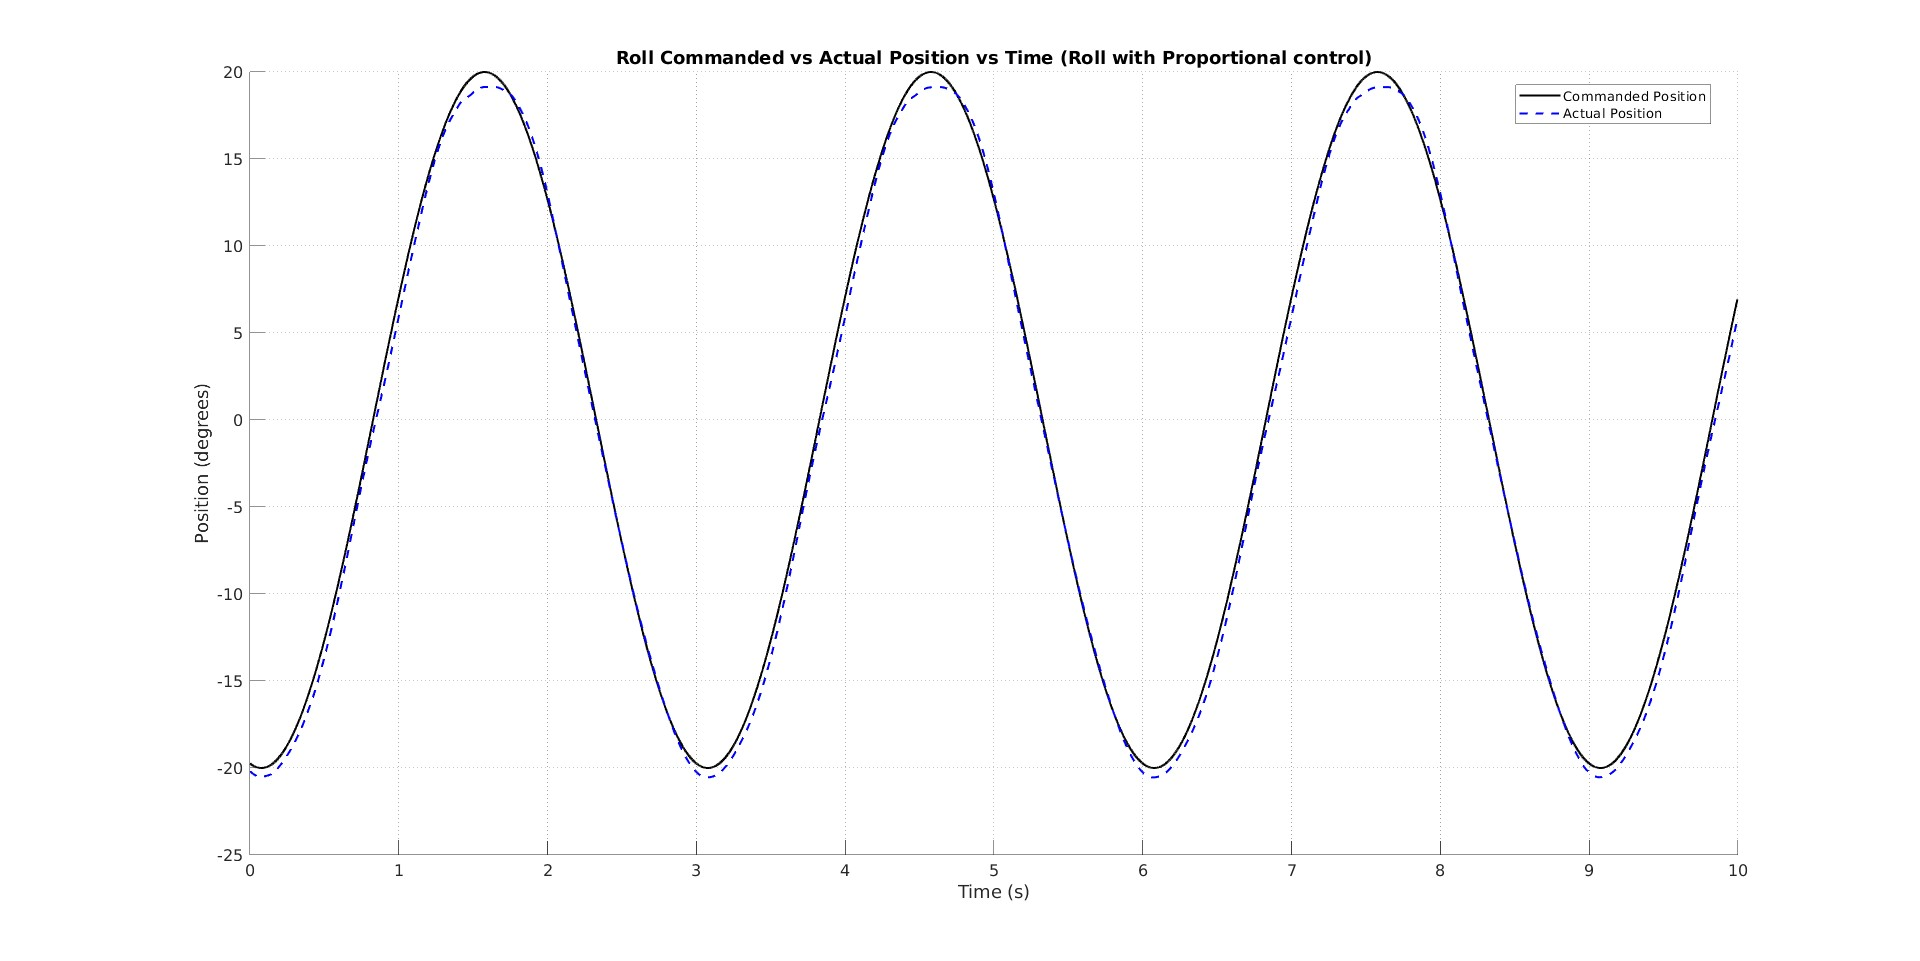
\includegraphics[width=1.0\linewidth]{figures/roll_p_sin.jpg}
    \caption{Sinusoidal path following performance of the Roll axis with proportional control, showing significant lag and overshoot.}
    \label{fig:roll_p_sin}
\end{figure}

\begin{figure}[H]
    \centering
    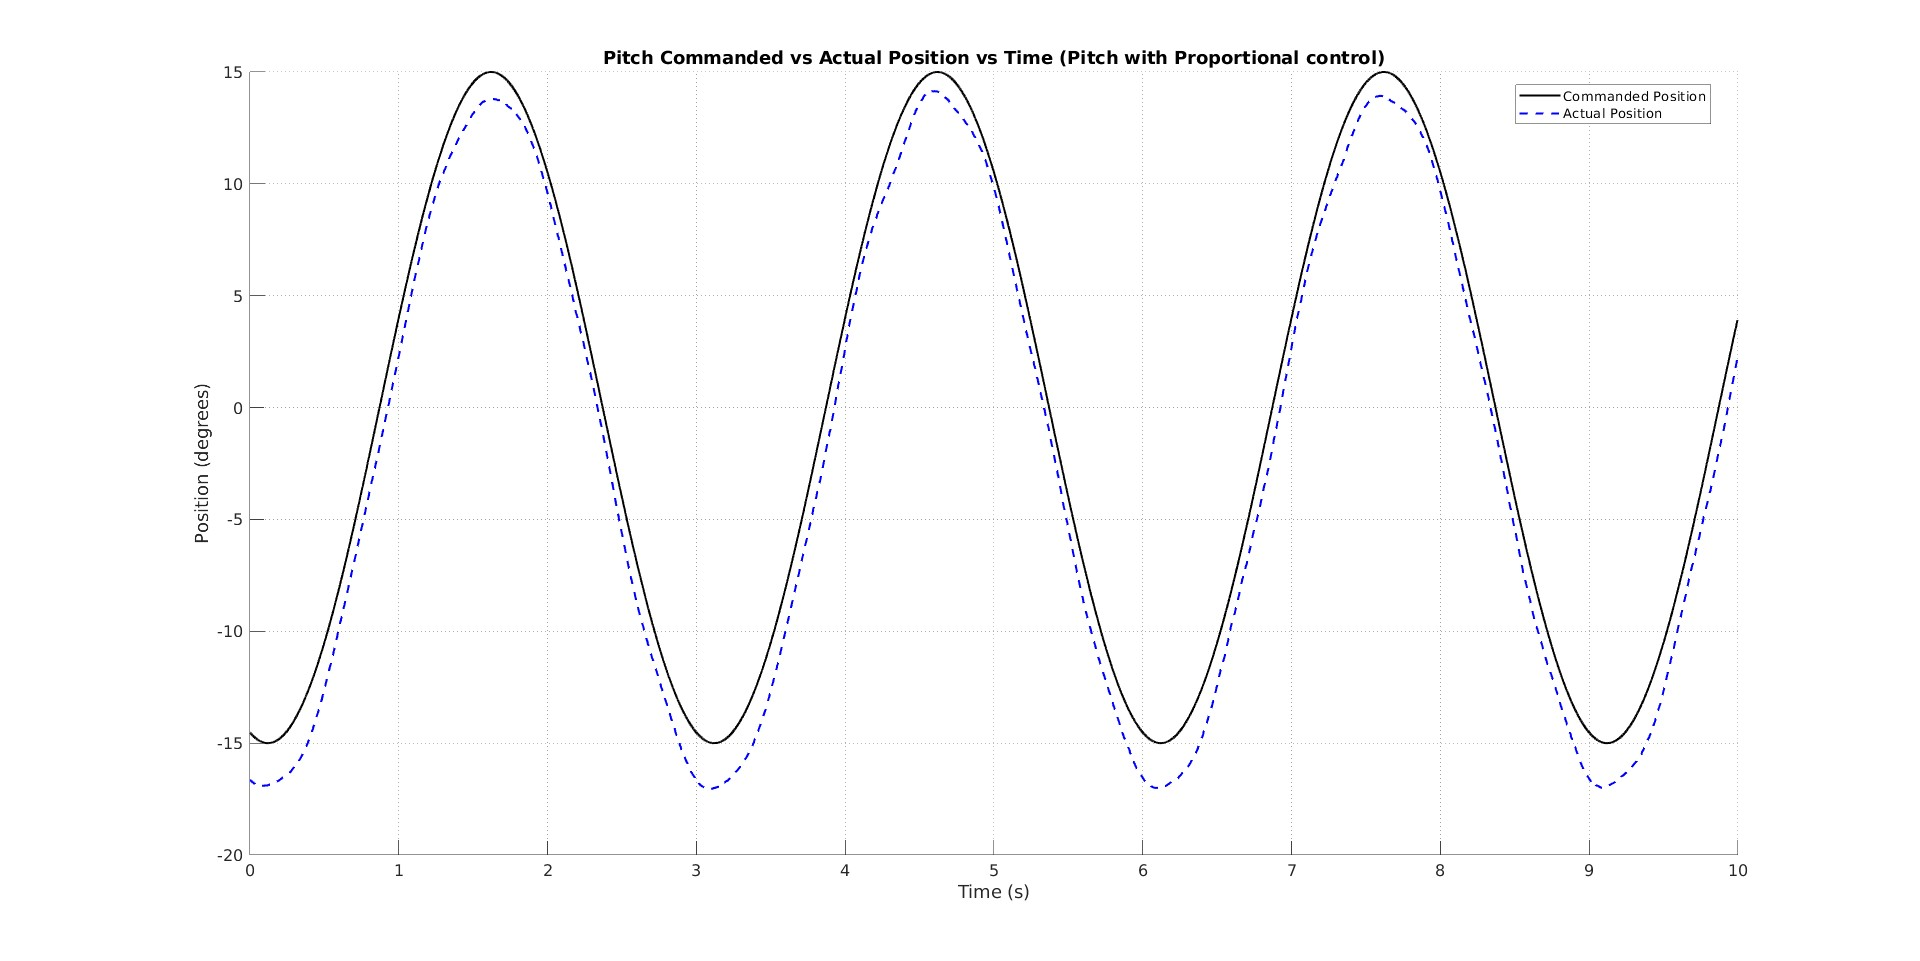
\includegraphics[width=1.00\linewidth]{figures/pitch_p_sin.jpg}
    \caption{Sinusoidal path following performance of the Pitch axis with proportional control, illustrating substantial undershoot and lag.}
    \label{fig:pitch_p_sin}
\end{figure}

The performance of the new control algorithm for sinusoidal path following was excellent. The system consistently followed the sinusoidal path with little to no lag, undershoot, or overshoot. This can clearly be seen in Figure \ref{fig:pitch_lqi_sin} and Figure \ref{fig:roll_lqr_sin}, where there is almost no noticeable difference between the commanded position and the actual position.

\begin{figure}[H]
    \centering
    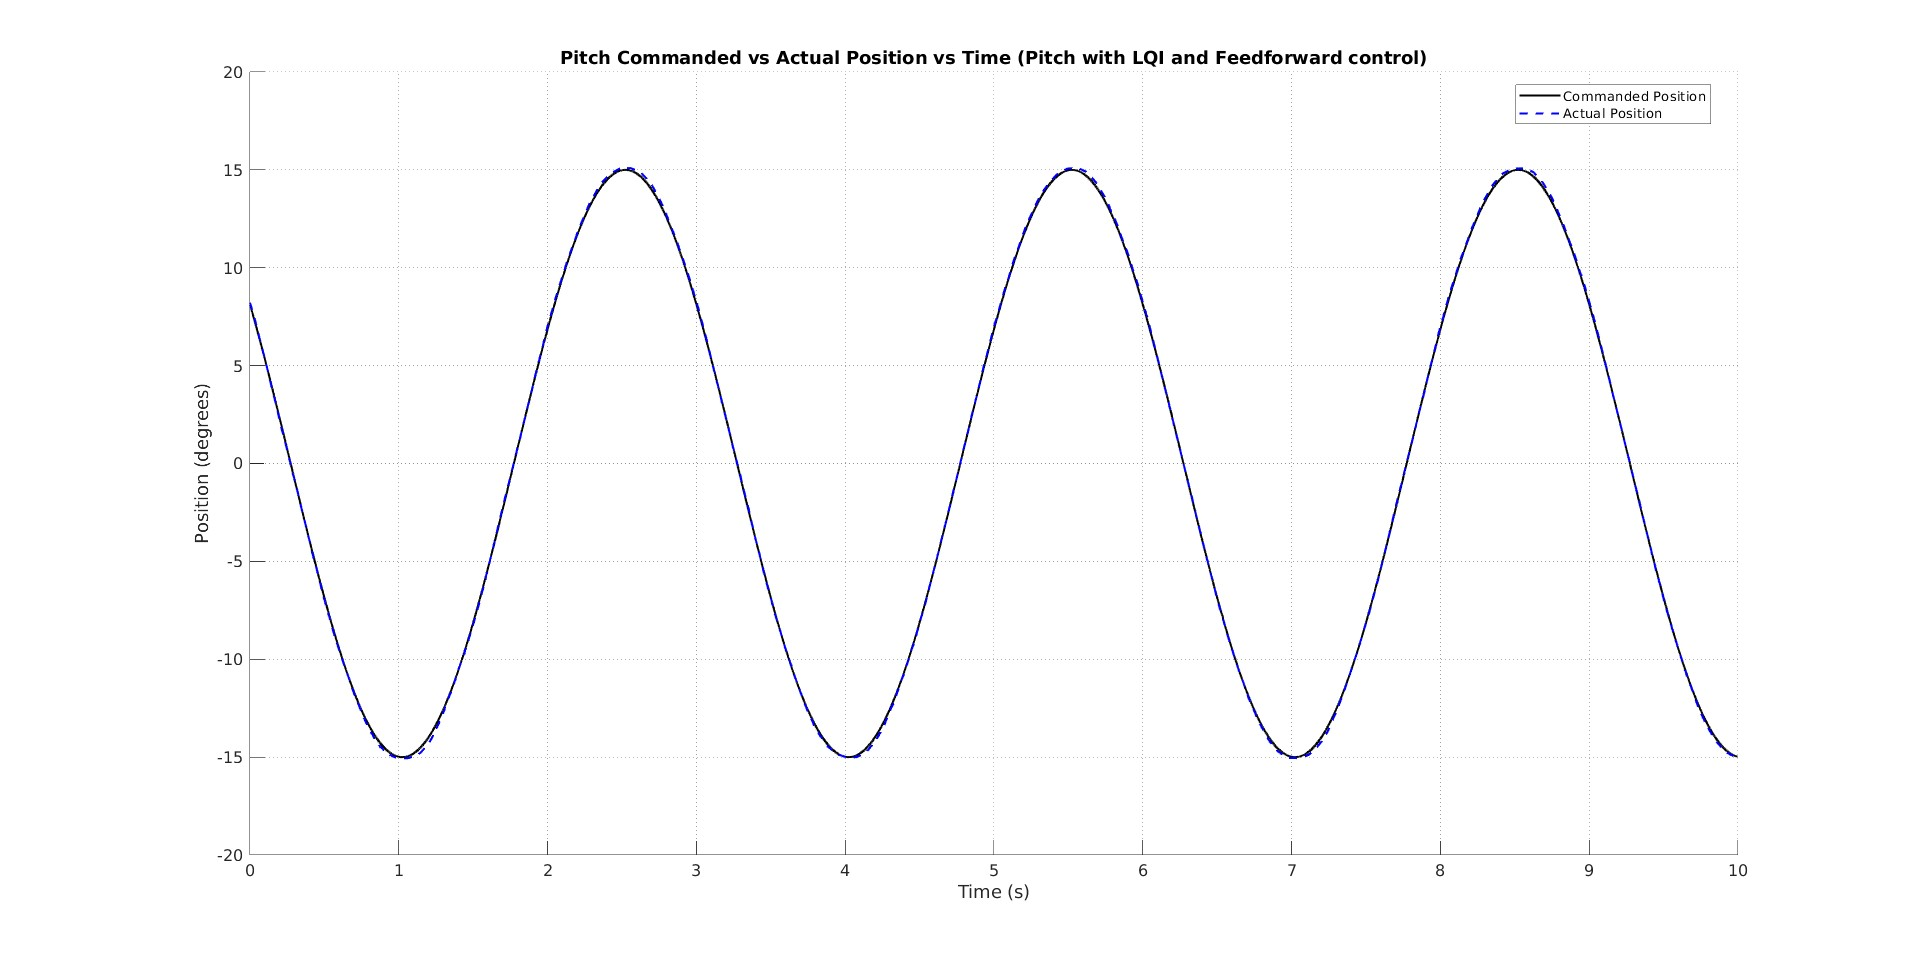
\includegraphics[width=1.00\linewidth]{figures/pitch_lqi_sin.jpg}
    \caption{Sinusoidal path following performance of the Pitch axis with the new LQI control algorithm, demonstrating excellent tracking with minimal error.}
    \label{fig:pitch_lqi_sin}
\end{figure}

\begin{figure}[H]
    \centering
    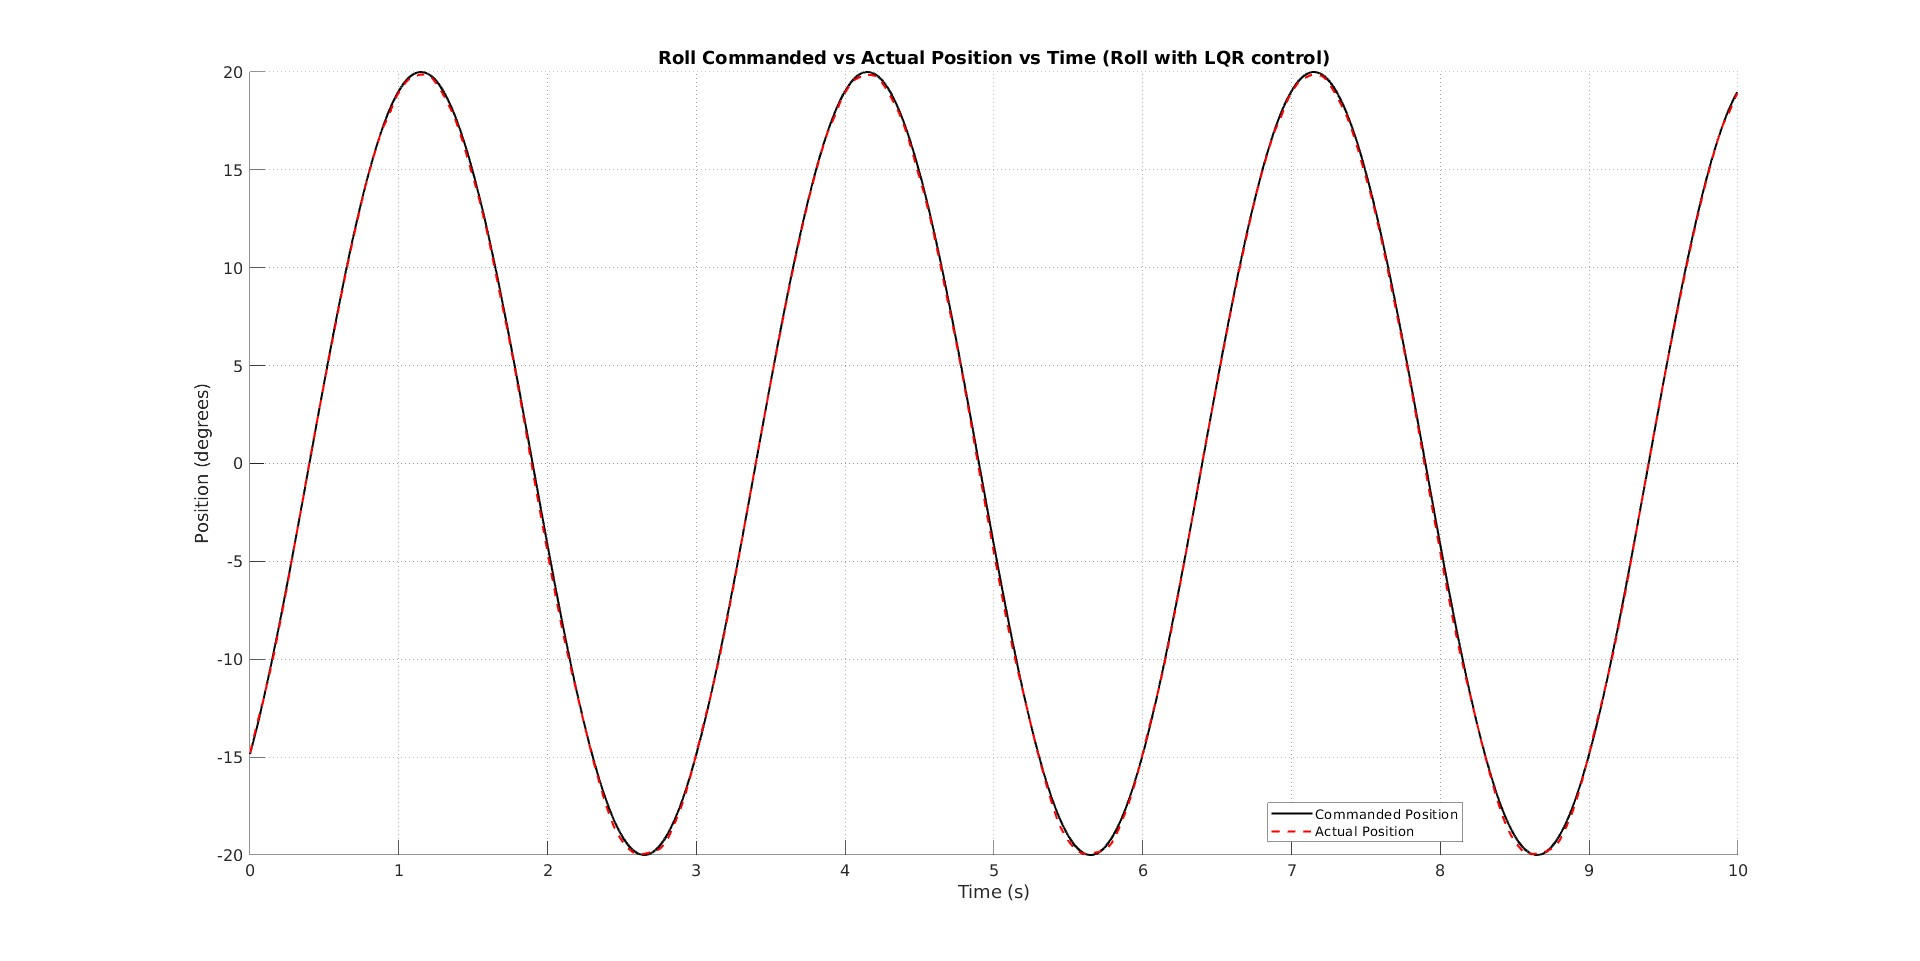
\includegraphics[width=1.00\linewidth]{figures/roll_lqr_sin.jpg}
    \caption{Sinusoidal path following performance of the Roll axis with the new LQR control algorithm, showing near-perfect tracking.}
    \label{fig:roll_lqr_sin}
\end{figure}

With the proportional control algorithm, the error in the pitch axis reached a maximum value of \SI{2.31}{\degree}, while the error in the roll axis reached \SI{1.17}{\degree}. The overall average error for the pitch axis was \SI{1.52}{\degree}, and the overall average error for the roll axis was \SI{0.62}{\degree}. These errors were particularly pronounced at the extrema of the joint angles, where the system struggled to maintain accuracy and stability.

With the new LQR and LQI with feedforward control algorithm, the maximum error in the pitch axis was reduced to \SI{0.35}{\degree}, and the maximum error in the roll axis was reduced to \SI{0.41}{\degree}. Both of these errors occurred at the extreme limits of their respective axes, and the average error of the pitch axis over the trial was \SI{0.12}{\degree}, while the value for the average error over the trial for the roll DOF was \SI{0.21}{\degree}.

The comparison of these errors between the control methods through the sinusoidal path following procedure can be seen in Figure \ref{fig:roll_sin_error} and Figure \ref{fig:pitch_sin_error}, where it is clear that the error for the new control method is much smaller than the older control method.

\begin{figure}[H]
    \centering
    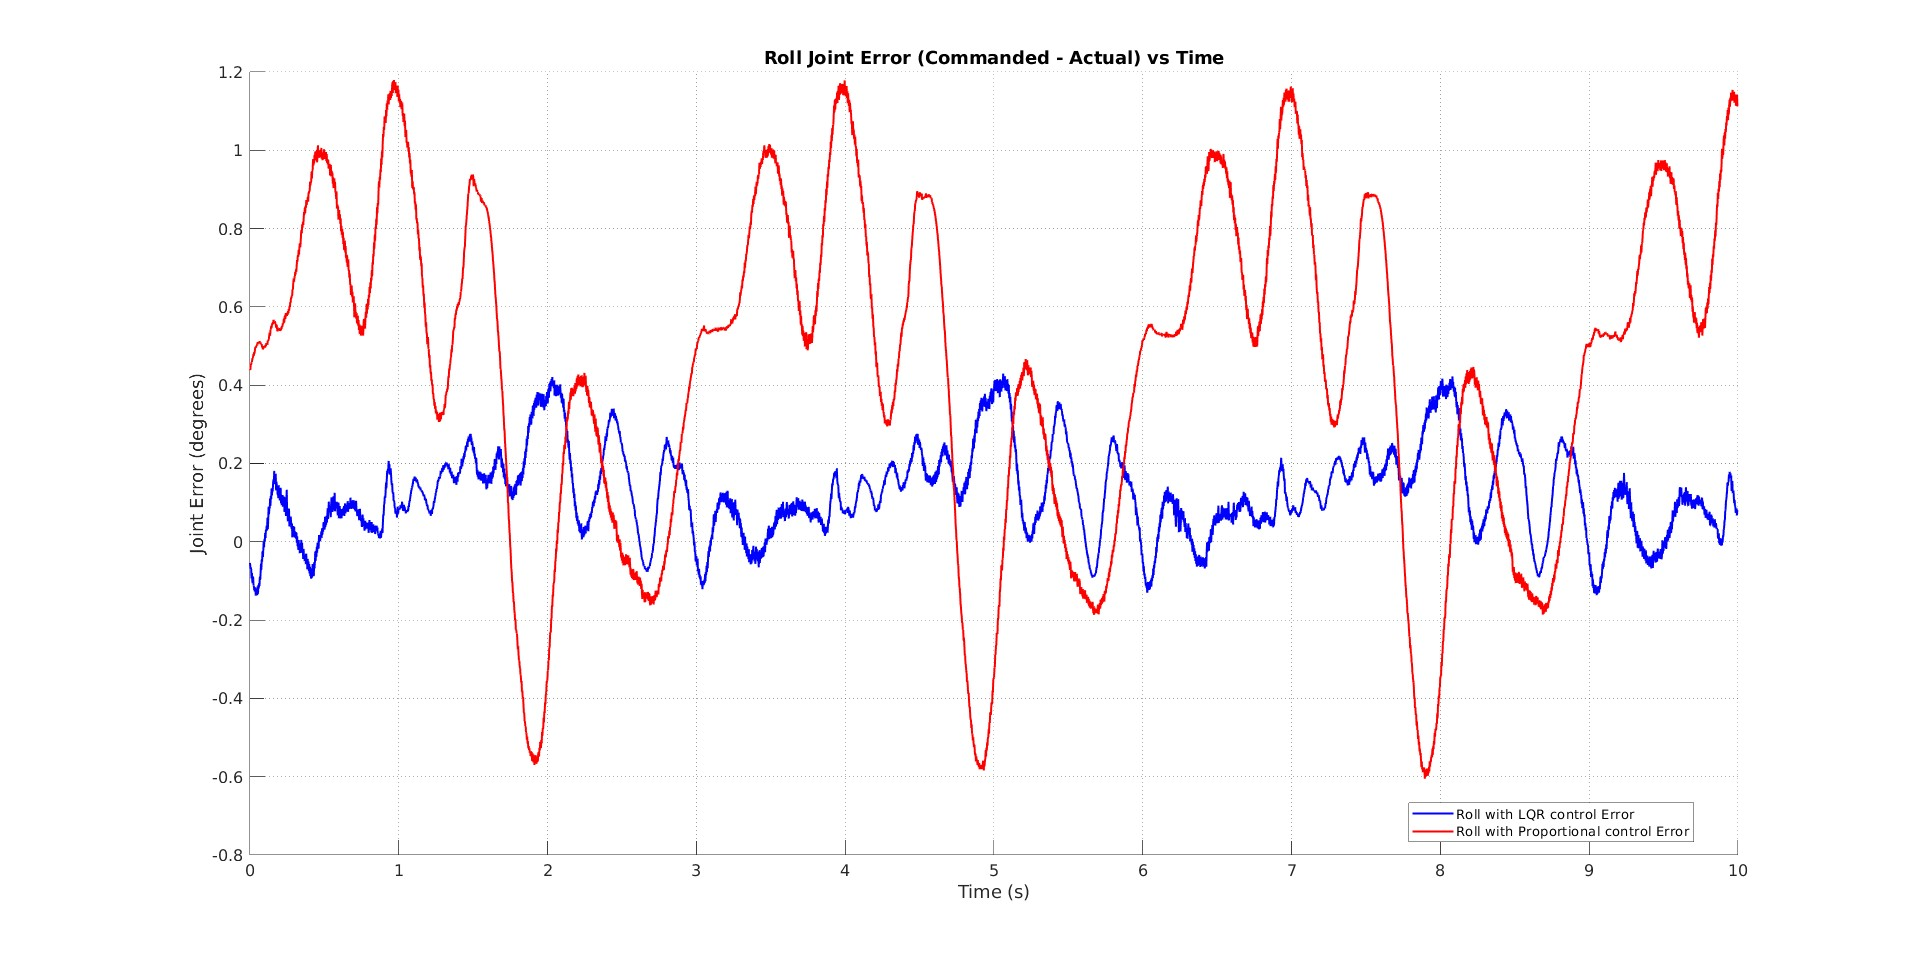
\includegraphics[width=1.00\linewidth]{figures/roll_sin_error.jpg}
    \caption{Comparison of Roll axis tracking error for proportional control vs. the new LQR control during sinusoidal path following.}
    \label{fig:roll_sin_error}
\end{figure}

\begin{figure}[H]
    \centering
    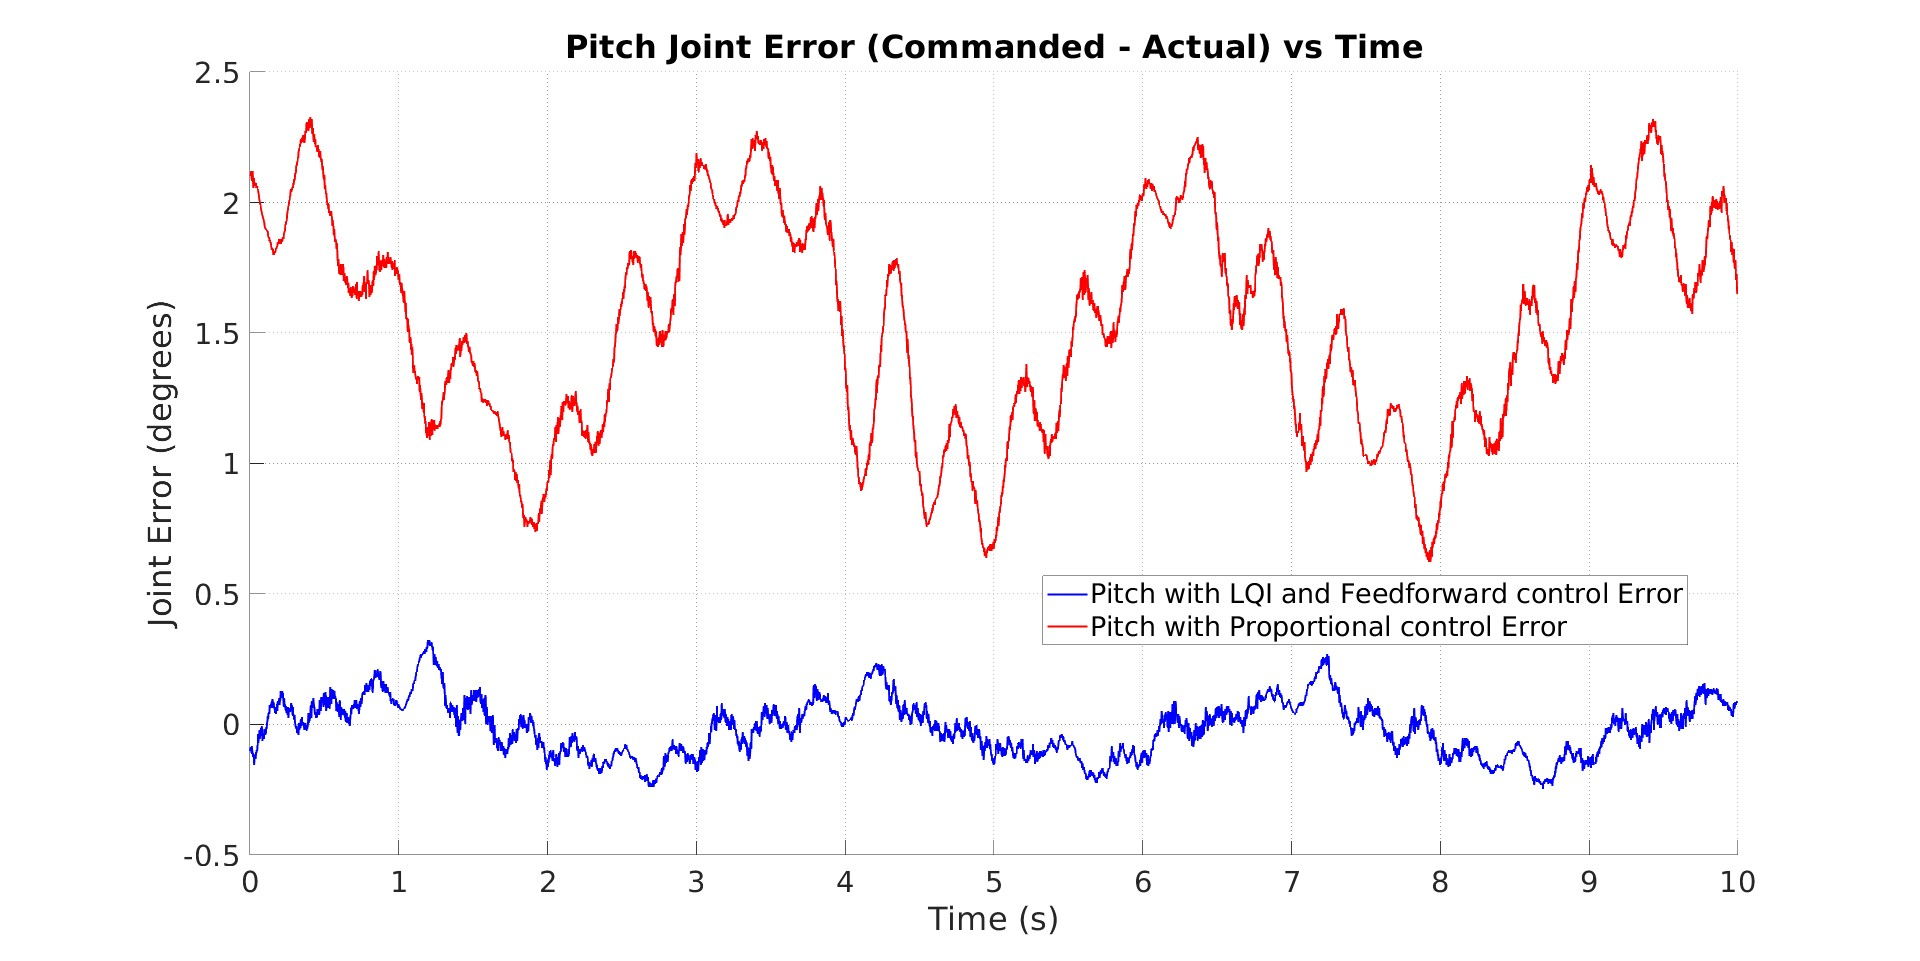
\includegraphics[width=1.00\linewidth]{figures/pitch_sin_error.jpg}
    \caption{Comparison of Pitch axis tracking error for proportional control vs. the new LQI control during sinusoidal path following.}
    \label{fig:pitch_sin_error}
\end{figure}

During sinusoidal path following, the new control algorithm's performance far exceeded that of the previous design. However, this procedure is not fully representative of real-world scenarios. During actual surgical procedures, the desired trajectory will very rarely be such a smooth, predictable path. As a result of this shortcoming, the system's performance following a real trajectory path must be examined.

\subsection{Target Following Experiment}

Similarly to the sinusoidal path following experiment, the new control algorithm's performance in the target path following experiment far exceeded that of the older control algorithm. This experiment used the 3D trajectory path shown in Figure \ref{fig:desired_trajectory}, which is representative of typical surgical movements.

\begin{figure}[H]
    \centering
    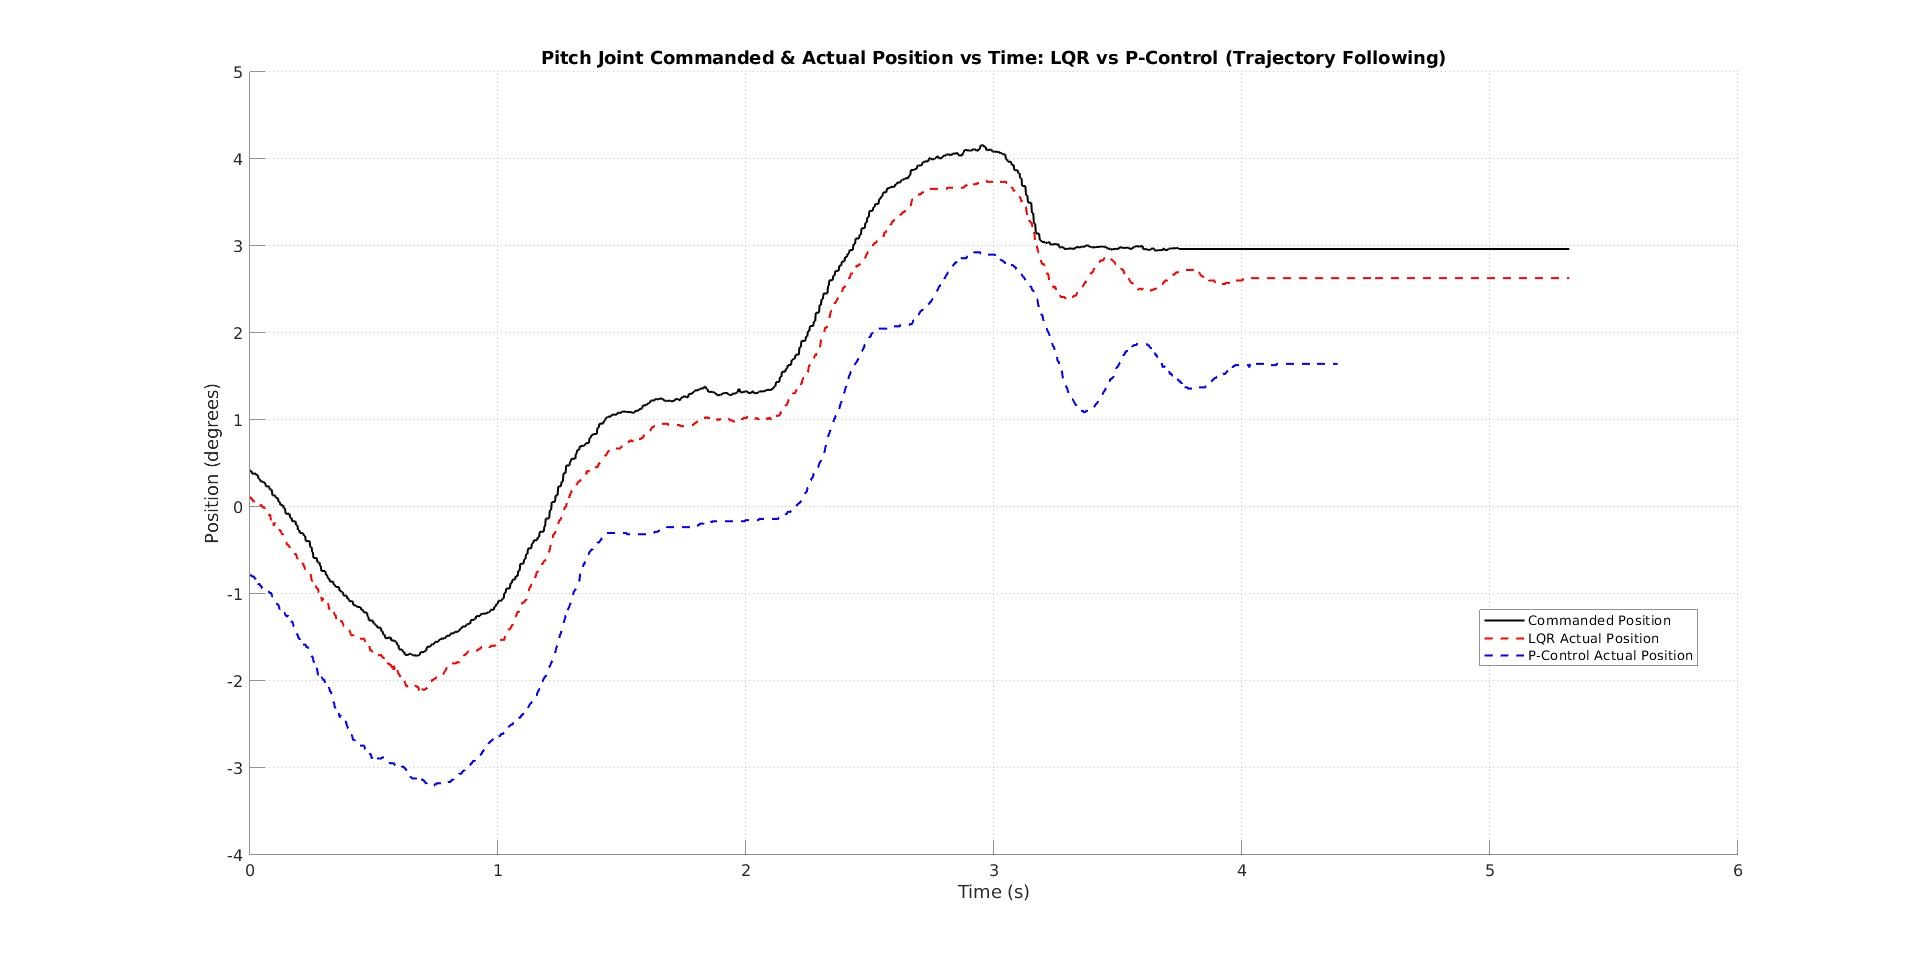
\includegraphics[width=1.00\linewidth]{figures/pitch_traj_combined.jpg}
    \caption{Target path following performance of the Pitch axis, comparing the old proportional control to the new LQI control algorithm. The new controller exhibits significantly improved tracking accuracy.}
    \label{fig:pitch_traj_combined}
\end{figure}

\begin{figure}[h!]
    \centering
    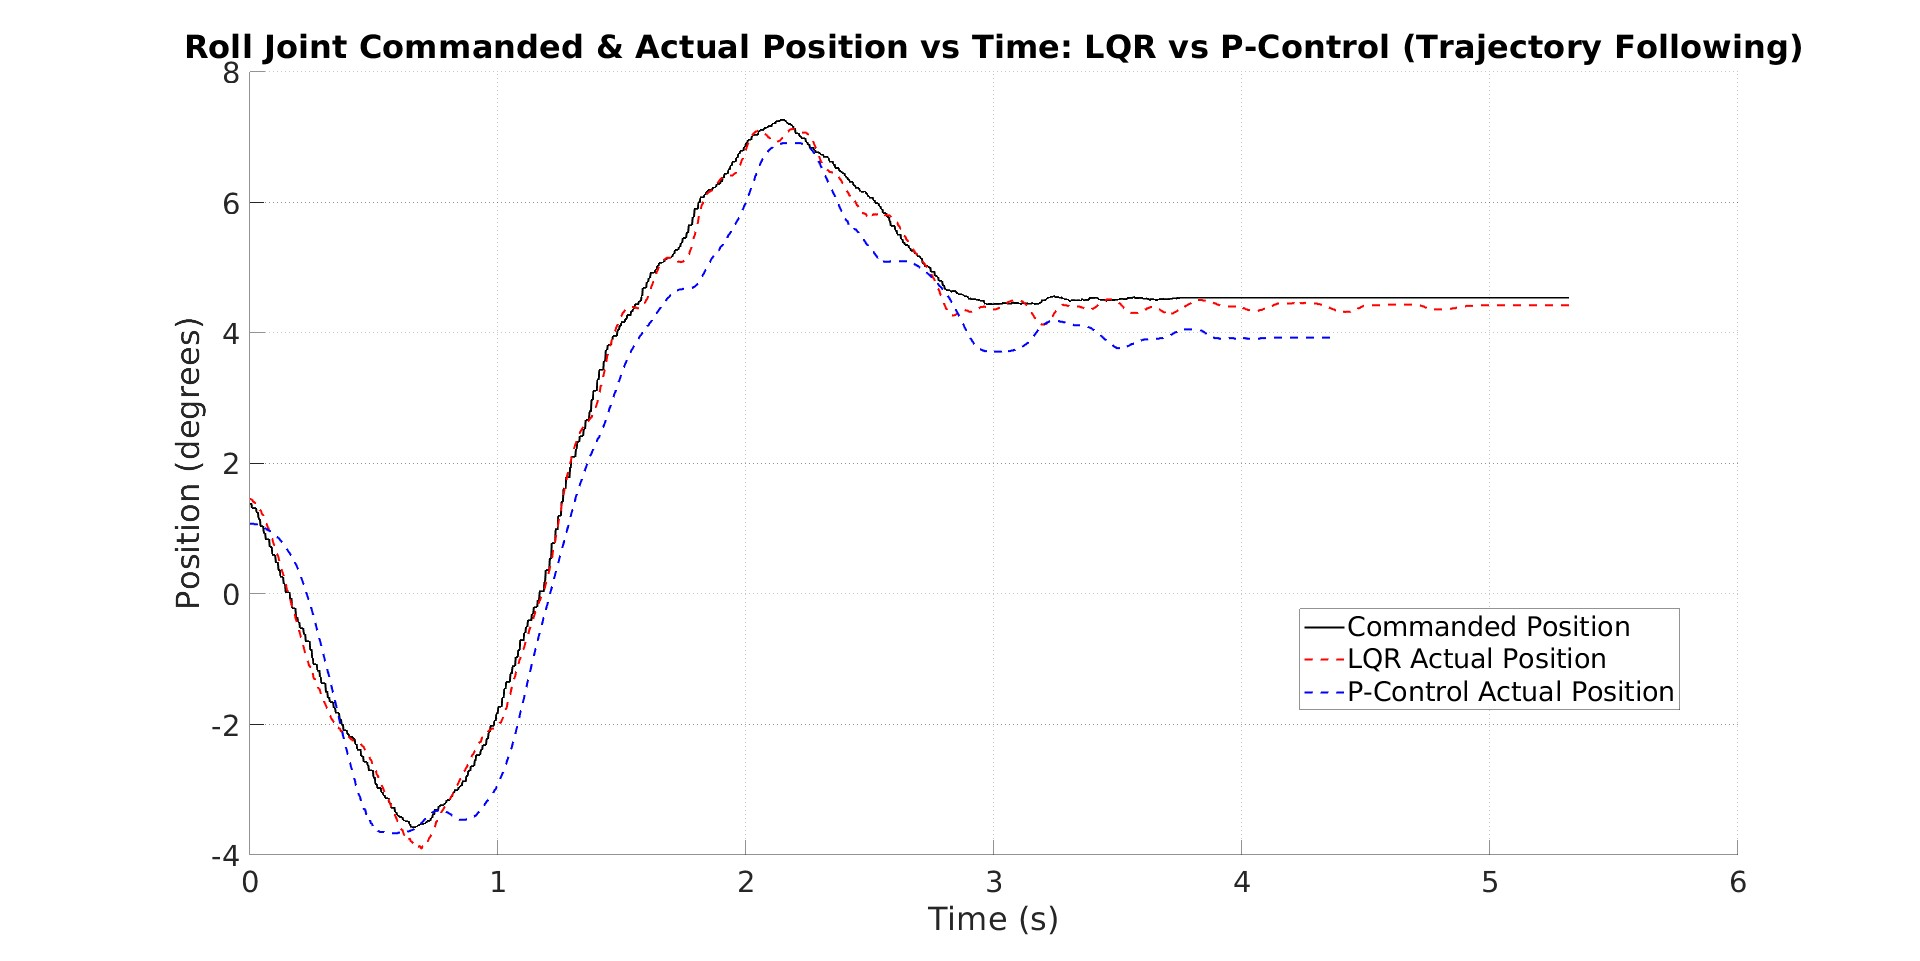
\includegraphics[width=1.00\linewidth]{figures/roll_traj_combined.jpg}
    \caption{Target path following performance of the Roll axis, comparing the old proportional control to the new LQR control algorithm. The new controller demonstrates superior tracking with reduced lag and overshoot.}
    \label{fig:roll_traj_combined}
\end{figure}

The reduction in error is clearly evident when comparing the old and new control methods. With the new LQR and LQI with feedforward control, the system maintained a much tighter adherence to the desired trajectory. This is visually represented in the error plots in Figure \ref{fig:roll_traj_error} and Figure \ref{fig:pitch_traj_error}, which show a substantial decrease in tracking error compared to the previous proportional control.

\begin{figure}[h!]
    \centering
    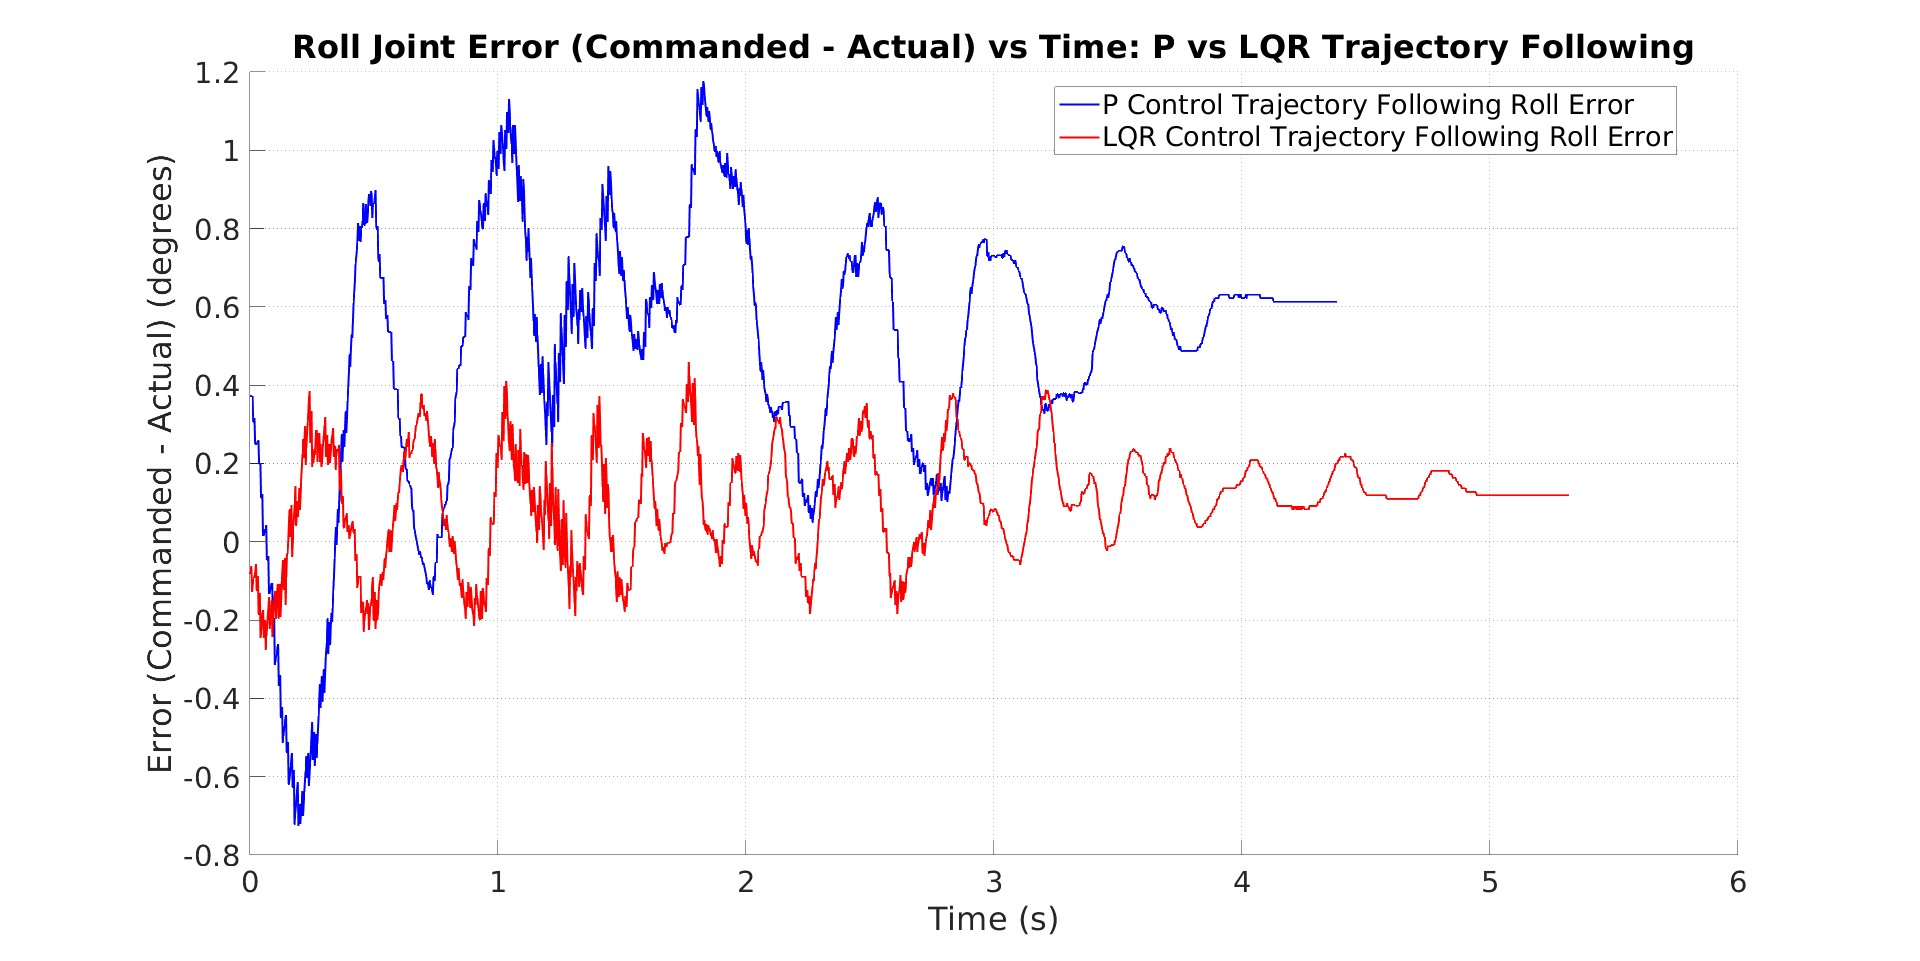
\includegraphics[width=1.00\linewidth]{figures/roll_traj_error.jpg}
    \caption{Comparison of Roll axis tracking error for proportional control vs. the new LQR control during complex target path following, highlighting the significant reduction in error with the new method.}
    \label{fig:roll_traj_error}
\end{figure}

\begin{figure}[h!]
    \centering
    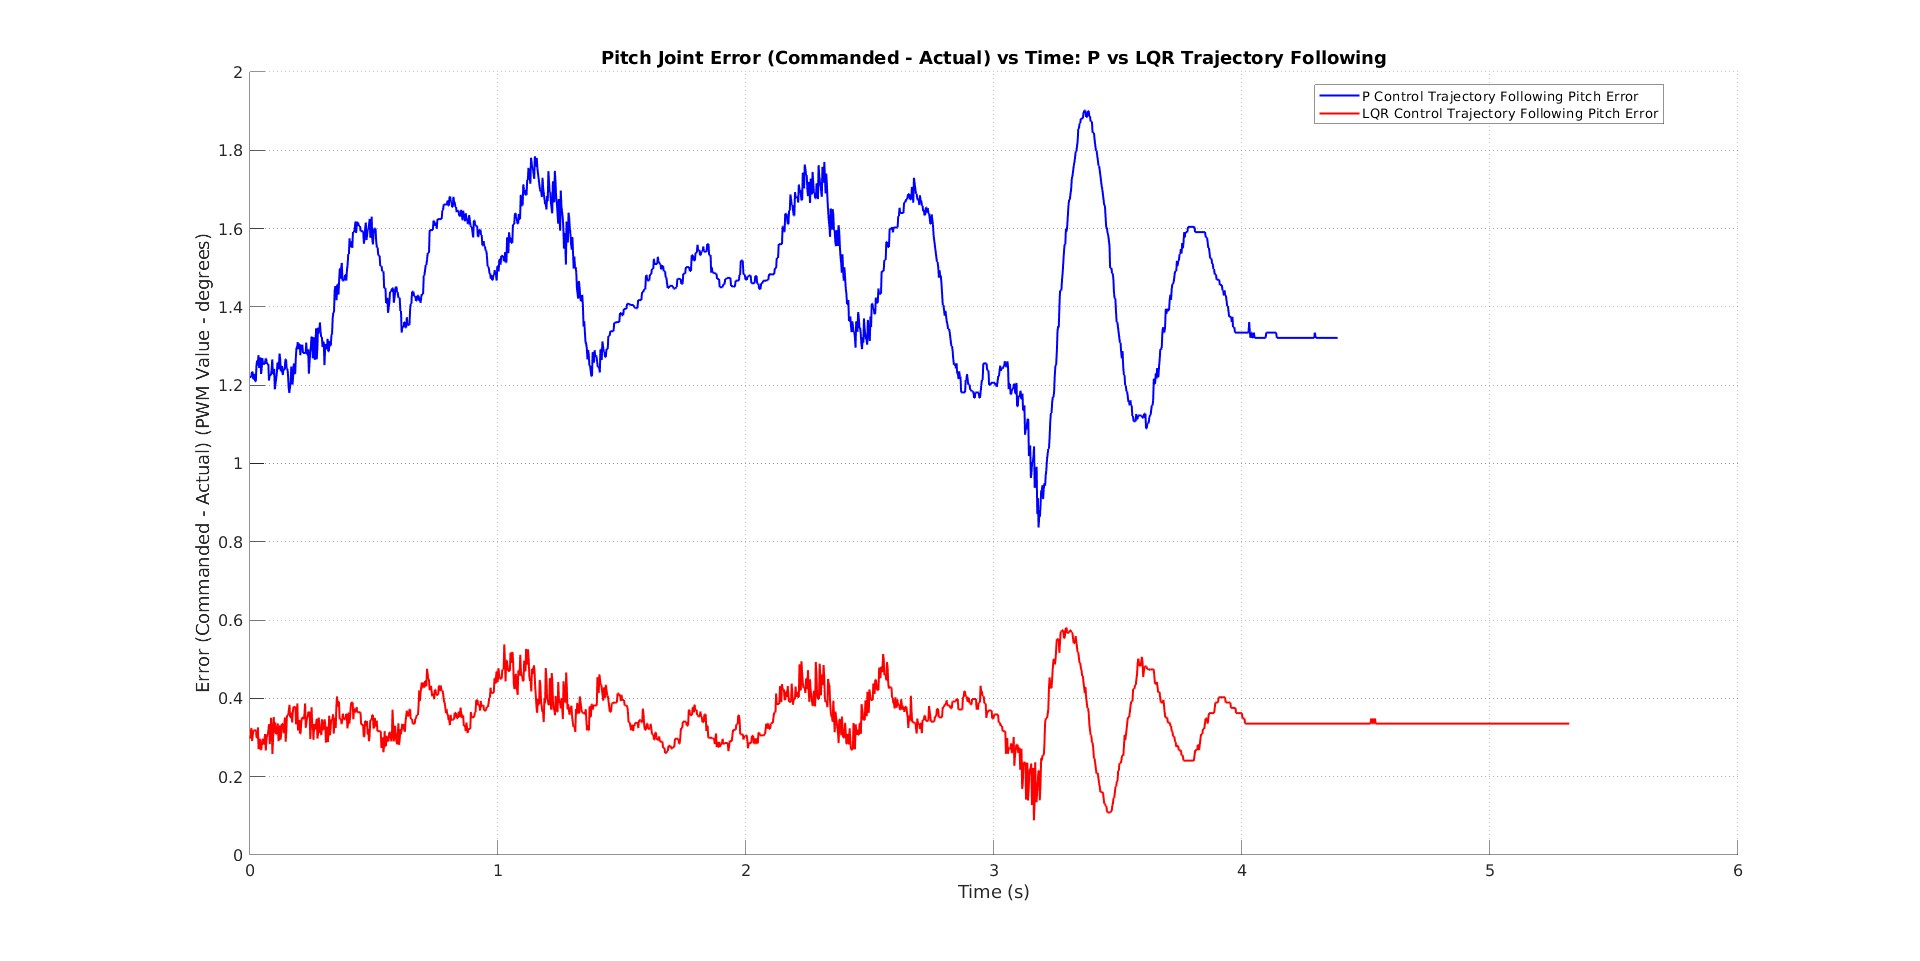
\includegraphics[width=1.0\linewidth]{figures/pitch_traj_error.jpg}
    \centering
    \caption{Comparison of Pitch axis tracking error for proportional control vs. the new LQI control during complex target path following, demonstrating improved accuracy with the updated algorithm.}
    \label{fig:pitch_traj_error}
\end{figure}